\documentclass[xcolor=dvipsnames,notes]{beamer}
\usecolortheme[named=Brown]{structure}
\usetheme{default}
\setbeamertemplate{navigation symbols}{} 
\usepackage{tikz}
\usetikzlibrary{arrows,decorations.pathmorphing,backgrounds,positioning,fit}
\usetikzlibrary{datavisualization.formats.functions}
\usetikzlibrary{shapes}
\usetikzlibrary{calc,patterns,angles,quotes}
%     
%Here are some macro's saving time and labour:     
%     
\newcommand{\const}{\mbox{const}}      
\newcommand{\est}{\mbox{{\tiny est}}}      
\newcommand{\im}{\mbox{$\Im \mbox{m}$}}      
\newcommand{\obs}{\mbox{{\tiny obs}}}      
\newcommand{\otherwise}{\mbox{otherwise}}      
\newcommand{\real}{\mbox{$\Re \mbox{e}$}}      
\newcommand{\sign}{\mbox{sign}}      
\newcommand{\sinc}{\mbox{sinc}}      
%
\newcommand{\p}{\mbox{$\partial$}}      
\renewcommand{\d}{\mbox{$\partial$}}      
\newcommand{\w}{\mbox{$\omega$}}      
%
\newcommand{\AAA}{\mbox{\boldmath $A$}}   
\newcommand{\BB}{\mbox{\boldmath $B$}}     
\newcommand{\CC}{\mbox{\boldmath $C$}}     
\newcommand{\DD}{\mbox{\boldmath $D$}}     
\newcommand{\EE}{\mbox{\boldmath $E$}}     
\newcommand{\FF}{\mbox{\boldmath $F$}}   
\newcommand{\GG}{\mbox{\boldmath $G$}}   
\newcommand{\HH}{\mbox{\boldmath $H$}}   
\newcommand{\II}{\mbox{\boldmath $I$}}   
\newcommand{\JJ}{\mbox{\boldmath $J$}}   
\newcommand{\KK}{\mbox{\boldmath $K$}}   
\newcommand{\LL}{\mbox{\boldmath $L$}}   
\newcommand{\MM}{\mbox{\boldmath $M$}}   
\newcommand{\NN}{\mbox{\boldmath $N$}}   
\newcommand{\OO}{\mbox{\boldmath $O$}}   
\newcommand{\PP}{\mbox{\boldmath $P$}}   
\newcommand{\QQ}{\mbox{\boldmath $Q$}}   
\newcommand{\RR}{\mbox{\boldmath $R$}}   
\newcommand{\SSS}{\mbox{\boldmath $S$}}   
\newcommand{\TT}{\mbox{\boldmath $T$}}   
\newcommand{\UU}{\mbox{\boldmath $U$}}   
\newcommand{\VV}{\mbox{\boldmath $V$}}   
\newcommand{\WW}{\mbox{\boldmath $W$}}   
\newcommand{\XX}{\mbox{\boldmath $X$}}   
\newcommand{\YY}{\mbox{\boldmath $Y$}}   
\newcommand{\ZZ}{\mbox{\boldmath $Z$}}   
%
%\newcommand{\aaa}{\mbox{\boldmath $a$}}     
\newcommand{\bb}{\mbox{\boldmath $b$}}     
\newcommand{\cc}{\mbox{\boldmath $c$}}     
\newcommand{\dd}{\mbox{\boldmath $d$}}     
\newcommand{\ee}{\mbox{\boldmath $e$}}   
\newcommand{\ff}{\mbox{\boldmath $f$}}   
%\newcommand{\ggg}{\mbox{\boldmath $g$}}   
\newcommand{\hh}{\mbox{\boldmath $h$}}   
\newcommand{\ii}{\mbox{\boldmath $i$}}   
\newcommand{\jj}{\mbox{\boldmath $j$}}   
\newcommand{\kk}{\mbox{\boldmath $k$}}   
%\newcommand{\lll}{\mbox{\boldmath $l$}}   
\newcommand{\mm}{\mbox{\boldmath $m$}}   
\newcommand{\nn}{\mbox{\boldmath $n$}}   
\newcommand{\pp}{\mbox{\boldmath $p$}}   
\newcommand{\qq}{\mbox{\boldmath $q$}}   
\newcommand{\rr}{\mbox{\boldmath $r$}}   
%\newcommand{\sss}{\mbox{\boldmath $s$}}   
%\newcommand{\ttt}{\mbox{\boldmath $t$}}   
\newcommand{\uu}{\mbox{\boldmath $u$}}   
\newcommand{\vv}{\mbox{\boldmath $v$}}   
\newcommand{\ww}{\mbox{\boldmath $w$}}   
\newcommand{\xx}{\mbox{\boldmath $x$}}   
\newcommand{\yy}{\mbox{\boldmath $y$}}   
\newcommand{\zz}{\mbox{\boldmath $z$}}   
%
\newcommand{\balpha}{\mbox{\boldmath $\alpha$}}     
\newcommand{\bpsi}{\mbox{\boldmath $\psi$}}     
\newcommand{\bphi}{\mbox{\boldmath $\phi$}}     
\newcommand{\bbeta}{\mbox{\boldmath $\beta$}}     
\newcommand{\btheta}{\mbox{\boldmath $\theta$}}     
\newcommand{\bdelta}{\mbox{\boldmath $\delta$}}     
\newcommand{\bgamma}{\mbox{\boldmath $d$}}     
\newcommand{\bGamma}{\mbox{\boldmath $\Gamma$}}     
\newcommand{\bLambda}{\mbox{\boldmath $\Lambda$}}     
\newcommand{\bmu}{\mbox{\boldmath $\mu$}}     
\newcommand{\bnabla}{\mbox{\boldmath $\nabla$}}     
\newcommand{\brho}{\mbox{\boldmath $\rho$}}     
\newcommand{\bSigma}{\mbox{\boldmath $\Sigma$}}     
\newcommand{\bsigma}{\mbox{\boldmath $\sigma$}}     
\newcommand{\bxi}{\mbox{\boldmath $\xi$}}     
\newcommand{\bepsilon}{\mbox{\boldmath $\epsilon$}}     
\newcommand{\blambda}{\mbox{\boldmath $\lambda$}}     
\newcommand{\BLambda}{\mbox{\boldmath $\Lambda$}}     
%-------------------------------------%
%  \Appendix - a new appendix command %
%-------------------------------------%
%The appendix command is used as in
% \Appendix{A}{The wave equation as a matrix equation}
\newcommand {\Appendix}[1]{
              \section*{APPENDIX #1}
              \setcounter{equation}{0}
              \renewcommand{\theequation} 
              {A-\arabic{equation}}}
\newcommand {\Appendices}[2]{
              \section*{APPENDIX #1: #2 }
              \setcounter{equation}{0}
              \renewcommand{\theequation} 
              {#1-\arabic{equation}}}
%------------------------------------%
%    \aref - a new cite command.     % 
%------------------------------------%
\newcommand{\aref}[2]{\nocite{#1}#2} 
%----------------------------------------
%\eqref -an equation reference command
%----------------------------------------
%\newcommand{\eqref}[1]{(\ref{#1})}
%\newcommand{\eqref}[1]{\ref{#1}}

\usepackage{epsfig}
\usepackage{natbib}
\usepackage{graphicx}
\usepackage{multimedia}
\usepackage{verbatim}
\include{acmmacro}
\begin{document}
%\setbeamercolor{titlelike}{fg=gray,bg=white}
%\setbeamercolor{itemize item}{fg=gray,bg=white}
%\setbeamercolor{enumerate item}{fg=gray,bg=white}
%\setbeamercolor{block title}{fg=black,bg=white}
%==============================================
\title{TPG4190 Seismic data acquisition and processing \\
               Lecture 15: Imaging 4 - Kirchoff and Angle migration}
\author{B. Arntsen}
\institute[NTNU]{
  NTNU\\
  Department of Geoscience and petroleum \\
  \texttt{borge.arntsen@ntnu.no}
}
\date{Trondheim fall 2020}
\begin{frame}
 \titlepage
\end{frame}
%
%==============================================
\begin{frame}{Overview}
%==============================================
\begin{itemize}
  \item State-of-the-art processing sequence
  \item The ray approximation
  \item The image formula usimg rays
  \item Kirchhoff migration
  \item Angle migration
  \item Kirchhoff computational cost
  \end{itemize}
\end{frame}
%---------------------------------------------------
\begin{frame}{State-of-the-art processing sequence}
%---------------------------------------------------
\begin{enumerate}
  \item Load data
  \item pre-processing
  \item Multiple removal
  \item Velocity estimation
  \item \textbf{Kirchoff Migration}
  \item Computation of angle gathers
  \item Residual corrections 
  \item Residual multiple removal
  \item Final filters
  \item Output of stacks, gathers
\end{enumerate}
\end{frame}
%---------------------------------------------------
\begin{frame}{The ray approximation}
%---------------------------------------------------
An apperoximate solution of the wave equation can be
found by assuming that thye solution is of a special form.
%
\begin{eqnarray}
\nabla^2 p(\xx,t) - \frac{1}{c^2(\xx)}\partial^2_t p(\xx,t) = 0
\end{eqnarray}
%
In the frequency domain we have
\begin{eqnarray}
\nabla^2 P(\xx,\omega) + \frac{\omega^2}{c^2(\xx)}\partial^2_t P(\xx,\omega) = 0
                                 \label{eq:waveq}
\end{eqnarray}

Now assume that
\begin{eqnarray}
  P(\xx,\omega) = A(\xx)\exp[i\omega\tau(\xx)]
                      \label{eq:ray}
\end{eqnarray}  
Here $A$ is the position-dependent Amplitude of $P$ 
wile $\tau$ is the position-dependent travel time.
\end{frame}
%---------------------------------------------------
\begin{frame}{The ray approximation}
%---------------------------------------------------
We want to insert the ray approximation (\eqref{eq:ray}) into
the wave equation (\eqref{eq:waveq}) to obtain equations for $A$ and $\tau$.
First compute $\nabla P$:
\begin{eqnarray}
\nabla P(\xx,\omega) = \nabla A(\xx)\exp[i\omega\tau(\xx)] 
		       + A(\xx)[i\omega\nabla\tau(\xx)]\exp[i\omega\tau(\xx)].
\end{eqnarray}
\begin{eqnarray}
\nabla[\nabla P(\xx,\omega)] = \nabla A^2(\xx)\exp[i\omega\tau(\xx)] 
                             + \nabla A(\xx)[i\omega\nabla\tau(\xx)]\exp[i\omega\tau(\xx)] \nonumber\\
                             + \nabla A(\xx)[i\omega\nabla\tau(\xx)\exp[i\omega\tau(\xx)] 
                             + A(\xx)(i\omega\nabla^2\tau(\xx)\exp[i\omega\tau(\xx)]       \nonumber \\
                             + A(\xx)[-\omega^2(\nabla\tau(\xx))^2\exp[i\omega\tau(\xx)].
\end{eqnarray}
\end{frame}
%---------------------------------------------------
\begin{frame}{The ray approximation}
%---------------------------------------------------
\begin{eqnarray}
\lefteqn{\nabla^2 P(\xx,\omega) +\omega^2/c^2(\xx)P(\xx,\omega)  = }& &  \\
                             &   & \nabla A^2(\xx)\exp[i\omega\tau(\xx)] \nonumber\\
                             & + & 2\nabla A(\xx)(i\omega\nabla\tau(\xx))\exp[i\omega\tau(\xx)] \nonumber\\
                             & + & A(\xx)(i\omega\nabla^2\tau(\xx)\exp[i\omega\tau(\xx)] \nonumber\\      
                             & + & A(\xx)[-\omega^2(\nabla\tau(\xx))^2\exp[i\omega\tau(\xx)]\nonumber\\
                             & + & A(\xx)\exp[i(\omega\tau(\xx)]\omega^2/c^2(\xx)\nonumber\\
                             & = & 0
\end{eqnarray}
Divide by $\omega^2$ to obtain:
\end{frame}
%---------------------------------------------------
\begin{frame}{The ray approximation}
%---------------------------------------------------
\begin{eqnarray}
                             & &\frac{1}{\omega^2}\nabla A^2(\xx)\exp[i\omega\tau(\xx)] \nonumber\\
                             & + & \frac{1}{\omega^2}2\nabla A(\xx)(i\omega\nabla\tau(\xx))\exp[i\omega\tau(\xx)] \nonumber\\
                             & + & \frac{1}{\omega^2}A(\xx)(i\omega\nabla^2\tau(\xx)\exp[i\omega\tau(\xx)] \nonumber\\      
                             & - & A(\xx)(\nabla\tau(\xx))^2\exp[i\omega\tau(\xx)]\nonumber\\
                             & + & A(\xx)\exp[i(\omega\tau(\xx)]1/c^2(\xx)\nonumber\\
                             & = & 0
\end{eqnarray}
\end{frame}
%---------------------------------------------------
\begin{frame}{The ray approximation}
%---------------------------------------------------
\begin{eqnarray}
                             & &\frac{1}{\omega^2}\nabla A^2(\xx) \nonumber\\
                             & + & \frac{1}{\omega^2}2\nabla A(\xx)(i\omega\nabla\tau(\xx)) \nonumber\\
                             & + & \frac{1}{\omega^2}A(\xx)(i\omega\nabla^2\tau(\xx)\nonumber\\      
                             & - & A(\xx)(\nabla\tau(\xx))^2\nonumber\\
                             & + & A(\xx)/c^2(\xx)\nonumber\\
                             & = & 0
\end{eqnarray}
\end{frame}
%---------------------------------------------------
\begin{frame}{The ray approximation}
%---------------------------------------------------
\begin{eqnarray}
                             \frac{1}{\omega^2}\nabla A^2(\xx) 
                              +  \frac{1}{\omega^2}2\nabla A(\xx)(i\omega\nabla\tau(\xx)) \nonumber\\
                              +  \frac{1}{\omega^2}A(\xx)(i\omega\nabla^2\tau(\xx)\nonumber\\      
                              +  A(\xx)(\nabla\tau(\xx))^2-A(\xx)\frac{1}{c^2(\xx)} = 0\nonumber\\
\end{eqnarray}
In the limit $\omega \rightarrow \infty$ this reduces to
\begin{eqnarray}
                              (\nabla\tau(\xx))^2-\frac{1}{c^2(\xx)} = 0
\end{eqnarray}
The Eikonal equation.
\end{frame}
%---------------------------------------------------
\begin{frame}{The ray approximation}
%---------------------------------------------------
\begin{eqnarray}
\nabla\tau(\xx) \cdot \nabla\tau(\xx) = \frac{1}{c^2(\xx)}
\end{eqnarray}
Solution for $c(\xx) = c_0=constant$
\begin{eqnarray}
\tau(\xx) = r/c_0
\end{eqnarray}
where $r$ is the distance from the position of the source.
\end{frame}
%---------------------------------------------------
\begin{frame}{The ray approximation}
%---------------------------------------------------
\begin{eqnarray}
P(\xx,\omega) = A(\xx) \exp[i\omega\tau(\xx)]
\end{eqnarray}
In the time-domain this is
\begin{eqnarray}
P(\xx,t) = A(\xx) \delta[t-\tau(\xx)]
\end{eqnarray}
\end{frame}
%---------------------------------------------------
\begin{frame}{Kirchoff migration}
%---------------------------------------------------
We use Claerbouts approximate imaging formula
\begin{eqnarray}
R(\xx) = \sum_{\xx_s} \int dt\, p(\xx,t)p_0(\xx,t)
\end{eqnarray}
Using the expression for $p$ in the
previous slide we get
\begin{eqnarray}
R(\xx) = \sum_{\xx_s} \int dt\, A(\xx)p[\xx,t+\tau_s(\xx)]A(\xx)\delta(t-\tau_r(\xx)]
\end{eqnarray}
\begin{eqnarray}
R(\xx') = \sum_{\xx_s} A(\xx)A(\xx) p[\xx,\tau_r(\xx)+\tau_s(\xx)]
\end{eqnarray}
\begin{eqnarray}
R(\xx') \approx \sum_{\xx_s} p[\xx,\tau_r(\xx)+\tau_s(\xx)]
\end{eqnarray}
\end{frame}
%==============================================
\begin{frame}{Kirchhoff depth migration}
%==============================================
%
\begin{figure}
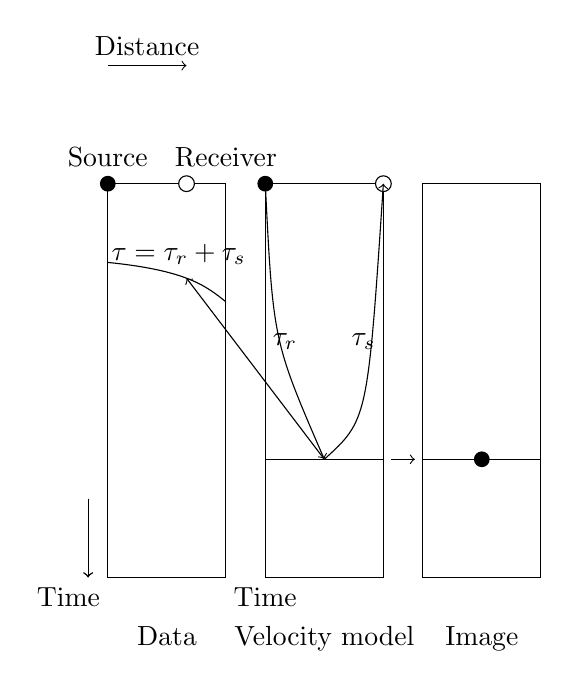
\begin{tikzpicture}[scale=1.0][stealth]
% Time section  
  \draw (0,0) rectangle +(1.5,5);
  \fill (0.0,5.0) circle (0.1) ;
  \draw (0.0,5.1) node[above]{Source};
  \fill[white] (1.0,5.0) circle (0.1) ;
  \draw (1.0,5.0) circle (0.1) ;
  \draw (1.5,5.1) node[above]{Receiver};
  \draw (0,4) .. controls (1.0,3.9) and (1.25,3.7).. (1.5,3.5);
  \draw (0.5,6.5) node[above]{Distance};
  \draw (-0.5,0) node[below]{Time};
  \draw[->] (0,6.5) -- (1,6.5);  
  \draw[->] (-0.25,1) -- (-0.25,0);  
  \draw (0.75,-0.5) node[below]{Data};
% Depth model
  \draw (2,0) rectangle +(1.5,5);
  \fill (2,0) +(0.0,5.0) circle (0.1) ;
  \fill[white] (2,0) +(1.5,5.0) circle (0.1) ;
  \draw (2,0) +(1.5,5.0) circle (0.1) ;
  \draw (2.0,0) node[below]{Time};
  %\draw[->] (0,5.5) -- (1,5.5);  
  \draw[->] (-0.25,1) -- (-0.25,0);  
%
% Rays
% \draw[->] (2.0,5) -- (2.75,1.5);
% \draw[->] (2.75,1.5) -- (3.5,5);

\draw[->] (2.0,5) .. controls (2.1, 3) ..(2.75,1.5);
  \draw[->] (2.75,1.5) .. controls (3.3,2.0) .. (3.5,5);
%
  \draw (2.0,1.5) -- (3.5,1.5);
  \draw (2,0) +(0.75,-0.5) node[below]{Velocity model};
  \draw (2,0) +(1.25,3) node{$\tau_s$};
  \draw (2,0) +(0.25,3) node{$\tau_r$};
  \draw[->] (2.75,1.5) -- (1.0,3.8);
  \draw (0.9,4.1) node{$\tau=\tau_r+\tau_s$};
% Image
  \draw[->] (3.6,1.5) -- (3.9,1.5);
  \draw (4,0) rectangle +(1.5,5);
  \draw (4,0) +(0.75,-0.5) node[below]{Image};
  \draw (4.0,1.5) -- +(1.5,0);
  \fill (4.75,1.5) circle (0.1) ;
\end{tikzpicture}
\caption{Kirchoff time migration}
\label{fig:si-4}
\end{figure}
\end{frame}
%
%------------------------------------------------
\begin{frame}{Common Image Point (CIP) Gathers}
%------------------------------------------------
%
\begin{figure}
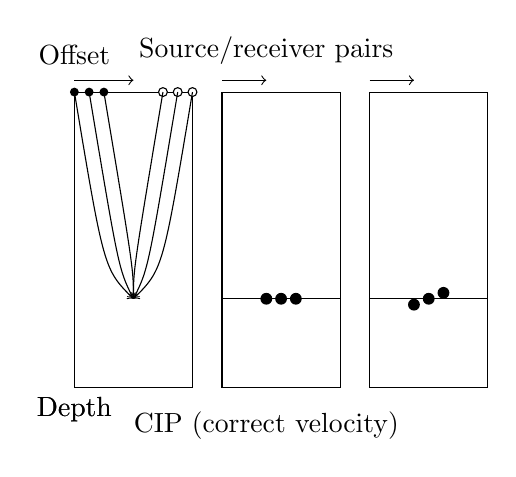
\begin{tikzpicture}[scale=0.75][stealth]
% Depth model outline
  \draw (0,0) rectangle +(2.0,5);
% Annotation on outline
  \draw[->] (0.0,5.2) -- +(1.0,0);
  \draw (0.0,5.3) node[above]{Offset};
  \draw (0.0,0) node[below]{Depth};
% Source point no1
  \fill (0,0) +(0.0,5.0) circle (0.075) ;
% Receiver point no1
  \fill[white] (0,0) +(2.0,5.0) circle (0.075) ;
  \draw (0,0) +(2.0,5.0) circle (0.075) ;
% Source point no2
  \fill (0,0) +(0.25,5.0) circle (0.075) ;
% Receiver point no2
  \fill[white] (0,0) +(1.75,5.0) circle (0.075) ;
  \draw (0,0) +(1.75,5.0) circle (0.075) ;
  \draw (0.0,0) node[below]{Depth};
% Source point no3
  \fill (0,0) +(0.5,5.0) circle (0.075) ;
% Receiver point no3
  \fill[white] (0,0) +(1.5,5.0) circle (0.075) ;
  \draw (0,0) +(1.5,5.0) circle (0.075) ;
% Ray pair no 1
  \draw[->] (0.0,5) .. controls (0.5,2.0) ..(1.0,1.5);
  \draw[->] (2.0,5) .. controls (1.5,2.0) ..(1.0,1.5);
% Ray pair no 2
  \draw[->] (0.25,5) .. controls (0.75,2.0) ..(1.0,1.5);
  \draw[->] (1.75,5) .. controls (1.25,2.0) ..(1.0,1.5);
% Ray pair no 2
  \draw[->] (0.5,5) .. controls (1.0,2.0) ..(1.0,1.5);
  \draw[->] (1.5,5) .. controls (1.0,2.0) ..(1.0,1.5);

% (Correct velocity)
%
% Common image points outline
  \draw (2.5,0) rectangle +(2.0,5);
% Common image points annotation
  \draw (2.5,5.3) +(0.75,0.0) node[above]{Source/receiver pairs};
  \draw[->] (2.5,5.2) -- +(0.75,0.0);
  \draw (2.5,0) +(0.75,-0.25) node[below]{CIP (correct velocity)};
% Horiz line
  \draw (2.5,1.5) -- (4.5,1.5);
% Common image point no 1 (center)
  \fill (3.5,1.5) circle (0.1) ;
% Common image point no 2 (left)
  \fill (3.25,1.5) circle (0.1) ;
% Common image point no 1 (right)
  \fill (3.75,1.5) circle (0.1) ;

%
% (Wrong velocity)
%
% Common image points outline
  \draw (5.0,0) rectangle +(2.0,5);
% Common image points annotation
  %\draw (5.0,5.3) +(0.75,0.0) node[above]{Source/receiver pairs};
  \draw[->] (5.0,5.2) -- +(0.75,0.0);
%  \draw (5.0,0) +(0.75,-0.25) node[below]{CIP (incorrect velocity)};
% Horiz line
  \draw (5.0,1.5) -- +(2.0,0.0);
% Common image point no 1 (center)
  \fill (6.0,1.5) circle (0.1) ;
% Common image point no 2 (left)
  \fill (5.75,1.4) circle (0.1) ;
% Common image point no 1 (right)
  \fill (6.25,1.6) circle (0.1) ;
\end{tikzpicture}
\caption{Common image-point gather}
\label{fig:si-300}
\end{figure}
\end{frame}
%==============================================
\begin{frame}{Kirchhoff time migration}
%==============================================
%
\begin{figure}
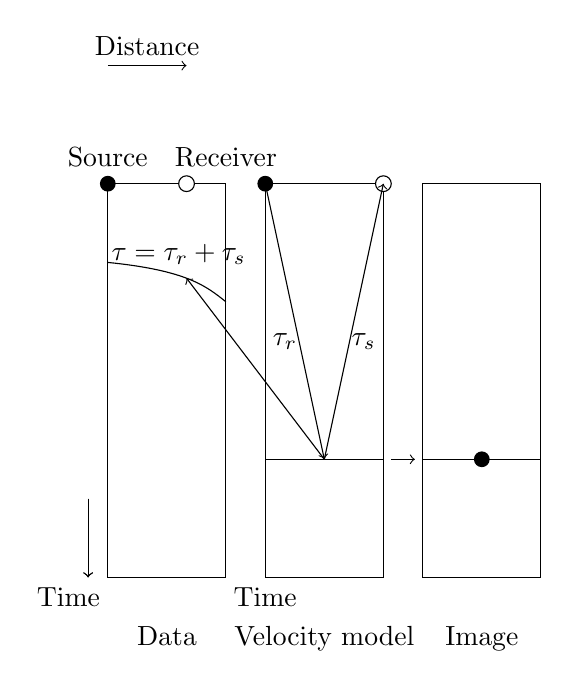
\begin{tikzpicture}[scale=1.0][stealth]
% Time section  
  \draw (0,0) rectangle +(1.5,5);
  \fill (0.0,5.0) circle (0.1) ;
  \draw (0.0,5.1) node[above]{Source};
  \fill[white] (1.0,5.0) circle (0.1) ;
  \draw (1.0,5.0) circle (0.1) ;
  \draw (1.5,5.1) node[above]{Receiver};
  \draw (0,4) .. controls (1.0,3.9) and (1.25,3.7).. (1.5,3.5);
  \draw (0.5,6.5) node[above]{Distance};
  \draw (-0.5,0) node[below]{Time};
  \draw[->] (0,6.5) -- (1,6.5);  
  \draw[->] (-0.25,1) -- (-0.25,0);  
  \draw (0.75,-0.5) node[below]{Data};
% Depth model
  \draw (2,0) rectangle +(1.5,5);
  \fill (2,0) +(0.0,5.0) circle (0.1) ;
  \fill[white] (2,0) +(1.5,5.0) circle (0.1) ;
  \draw (2,0) +(1.5,5.0) circle (0.1) ;
  \draw (2.0,0) node[below]{Time};
  %\draw[->] (0,5.5) -- (1,5.5);  
  \draw[->] (-0.25,1) -- (-0.25,0);  
%
% Rays
 \draw[->] (2.0,5) -- (2.75,1.5);
 \draw[->] (2.75,1.5) -- (3.5,5);

  \draw (2.0,1.5) -- (3.5,1.5);
  \draw (2,0) +(0.75,-0.5) node[below]{Velocity model};
  \draw (2,0) +(1.25,3) node{$\tau_s$};
  \draw (2,0) +(0.25,3) node{$\tau_r$};
  \draw[->] (2.75,1.5) -- (1.0,3.8);
  \draw (0.9,4.1) node{$\tau=\tau_r+\tau_s$};
% Image
  \draw[->] (3.6,1.5) -- (3.9,1.5);
  \draw (4,0) rectangle +(1.5,5);
  \draw (4,0) +(0.75,-0.5) node[below]{Image};
  \draw (4.0,1.5) -- +(1.5,0);
  \fill (4.75,1.5) circle (0.1) ;
\end{tikzpicture}
\caption{Kirchoff time migration}
\label{fig:si-5}
\end{figure}
\end{frame}
%==============================================
\begin{frame}{Angle migration}
%==============================================
%
\begin{figure}
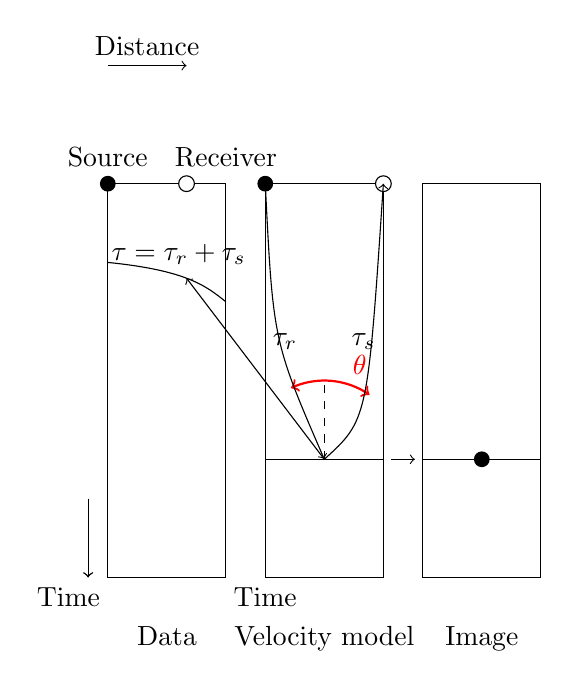
\begin{tikzpicture}[scale=1.0][stealth]
% Time section  
  \draw (0,0) rectangle +(1.5,5);
  \fill (0.0,5.0) circle (0.1) ;
  \draw (0.0,5.1) node[above]{Source};
  \fill[white] (1.0,5.0) circle (0.1) ;
  \draw (1.0,5.0) circle (0.1) ;
  \draw (1.5,5.1) node[above]{Receiver};
  \draw (0,4) .. controls (1.0,3.9) and (1.25,3.7).. (1.5,3.5);
  \draw (0.5,6.5) node[above]{Distance};
  \draw (-0.5,0) node[below]{Time};
  \draw[->] (0,6.5) -- (1,6.5);  
  \draw[->] (-0.25,1) -- (-0.25,0);  
  \draw (0.75,-0.5) node[below]{Data};
% Depth model
  \draw (2,0) rectangle +(1.5,5);
  \fill (2,0) +(0.0,5.0) circle (0.1) ;
  \fill[white] (2,0) +(1.5,5.0) circle (0.1) ;
  \draw (2,0) +(1.5,5.0) circle (0.1) ;
  \draw (2.0,0) node[below]{Time};
  %\draw[->] (0,5.5) -- (1,5.5);  
  \draw[->] (-0.25,1) -- (-0.25,0);  
%
% Rays
% \draw[->] (2.0,5) -- (2.75,1.5);
% \draw[->] (2.75,1.5) -- (3.5,5);
\draw[dashed] (2.75,1.5) -- (2.75,2.5);
\draw [<->,red,thick,domain=55:115] plot ({2.75+cos(\x)}, {1.5+sin(\x)});
\draw[->] (2.0,5) .. controls (2.1, 3) ..(2.75,1.5);
\draw[->] (2.75,1.5) .. controls (3.3,2.0) .. (3.5,5);
\node[red] at (3.2,2.70) {$\theta$}; 
 
%
  \draw (2.0,1.5) -- (3.5,1.5);
  \draw (2,0) +(0.75,-0.5) node[below]{Velocity model};
  \draw (2,0) +(1.25,3) node{$\tau_s$};
  \draw (2,0) +(0.25,3) node{$\tau_r$};
  \draw[->] (2.75,1.5) -- (1.0,3.8);
  \draw (0.9,4.1) node{$\tau=\tau_r+\tau_s$};
% Image
  \draw[->] (3.6,1.5) -- (3.9,1.5);
  \draw (4,0) rectangle +(1.5,5);
  \draw (4,0) +(0.75,-0.5) node[below]{Image};
  \draw (4.0,1.5) -- +(1.5,0);
  \fill (4.75,1.5) circle (0.1) ;
\end{tikzpicture}
\caption{Kirchoff time migration}
\label{fig:si-6}
\end{figure}
\end{frame}
%
\end{document}
